% Name: Call stack frames
% Description: Three frames on the stack, with the frame and stack pointers and a brace for each function.
% Tags: call stack, stack frame, compilers, assembly

\usetikzlibrary{arrows.meta, decorations.pathreplacing}

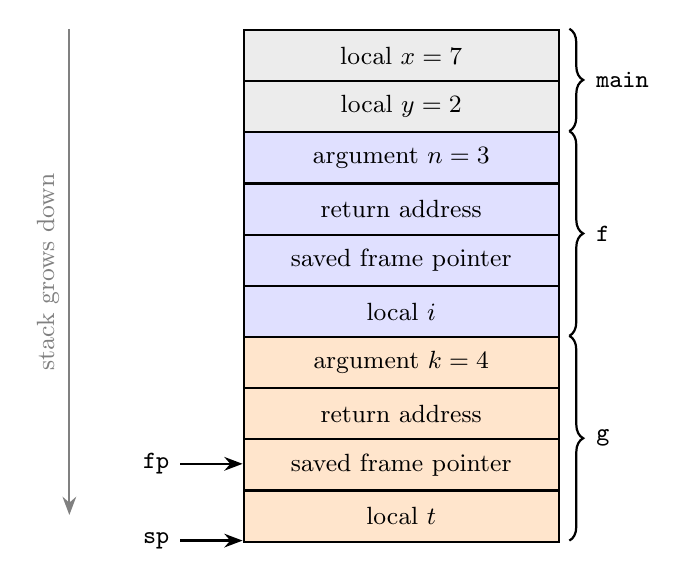
\begin{tikzpicture}[
  y=6.5mm, >={Stealth},
  every node/.style={font=\small},
  cell/.style={draw, thick, minimum width=40mm, minimum height=6.5mm, anchor=north west},
]
  \foreach \label/\fill [count=\i] in {
    {local $x = 7$}/gray!15, {local $y = 2$}/gray!15,
    {argument $n = 3$}/blue!12, {return address}/blue!12, {saved frame pointer}/blue!12, {local $i$}/blue!12,
    {argument $k = 4$}/orange!20, {return address}/orange!20, {saved frame pointer}/orange!20, {local $t$}/orange!20%
  }
    \node[cell, fill=\fill] at (0,-\i) {\label};

  \foreach \top/\bottom/\name in {1/3/main, 3/7/f, 7/11/g}
    \draw[decorate, decoration={brace, amplitude=5pt}, thick] (4.15,-\top) -- (4.15,-\bottom)
      node[midway, right=6pt] {\texttt{\name}};
  \draw[<-, thick] (0,-9.5) -- ++(-0.8,0) node[left] {\texttt{fp}};
  \draw[<-, thick] (0,-11) -- ++(-0.8,0) node[left] {\texttt{sp}};
  \draw[->, thick, gray] (-2.2,-1) -- (-2.2,-10.5) node[midway, above, rotate=90] {stack grows down};
\end{tikzpicture}
